\section{训练初期}
在学习鼠开始学习与行为交互相关的知识时,Q表均为其初始值0。这意味着其全部状态-动作组均需进行尝试,难以与规则鼠进行有效的行为交互。而从实际表现看,此阶段学习鼠的行为表现具有极大的随机性,运动方向和动作模式均与生物鼠表现存在较大差异,未能成功引发与规则鼠的交互行为。
\begin{figure}[htbp]
  \vspace{13pt}
  \centering
  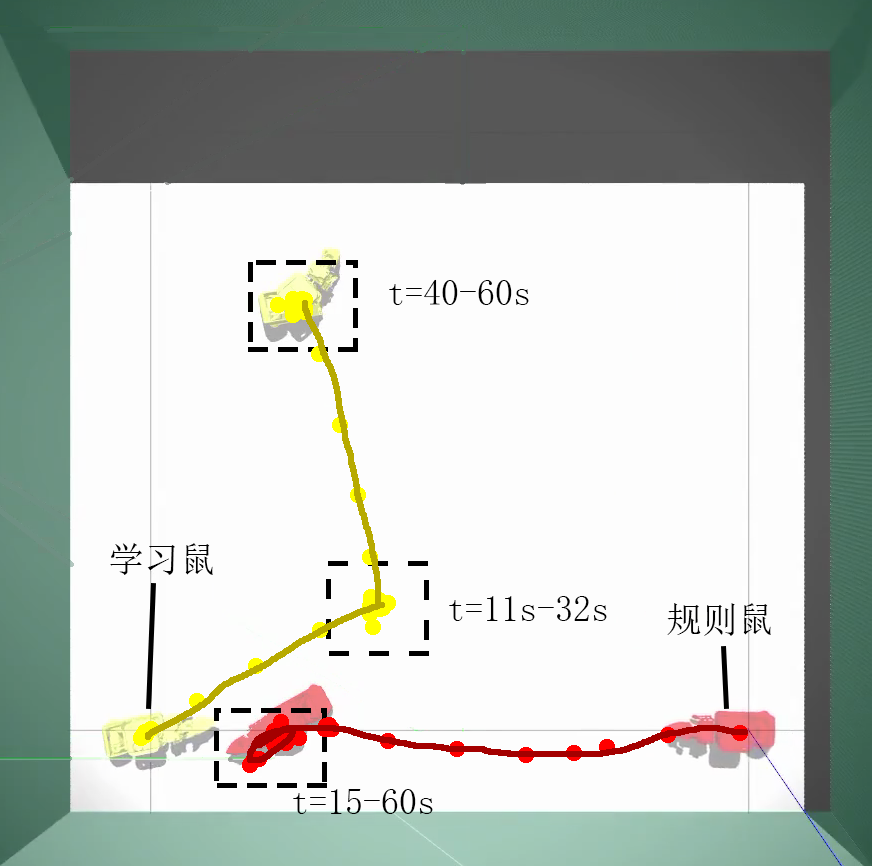
\includegraphics[height=6cm]{images/ch05/start/robotic/robotic.png}
  \caption{训练开始阶段机器鼠运动热点图及运动轨迹($1~min$)}\label{figure_roboticheatmap}
\end{figure}

图\ref{figure_roboticheatmap}展示了这一阶段$1~min$内仿生机器鼠在实验场景中运动的热点图及运动轨迹。由此图观察得知,在$0\sim15~s $内,规则鼠向学习鼠靠拢,尝试与学习鼠进行行为交互,但这一时期学习鼠并未习得任何行为交互的知识,处于完全的“探索”阶段,其动作序列随机生成,因此并未回应规则鼠的这一尝试交互的举动。随后,在$15\sim60~s$内,规则鼠陷入了较长时间“不交互”的状态,此时规则鼠倾向于在原处行动。
\begin{figure}[htbp]
  \vspace{13pt}
  \centering
  \subfigure[$t=11~s$]{\label{figure_startdirectionchange11}
  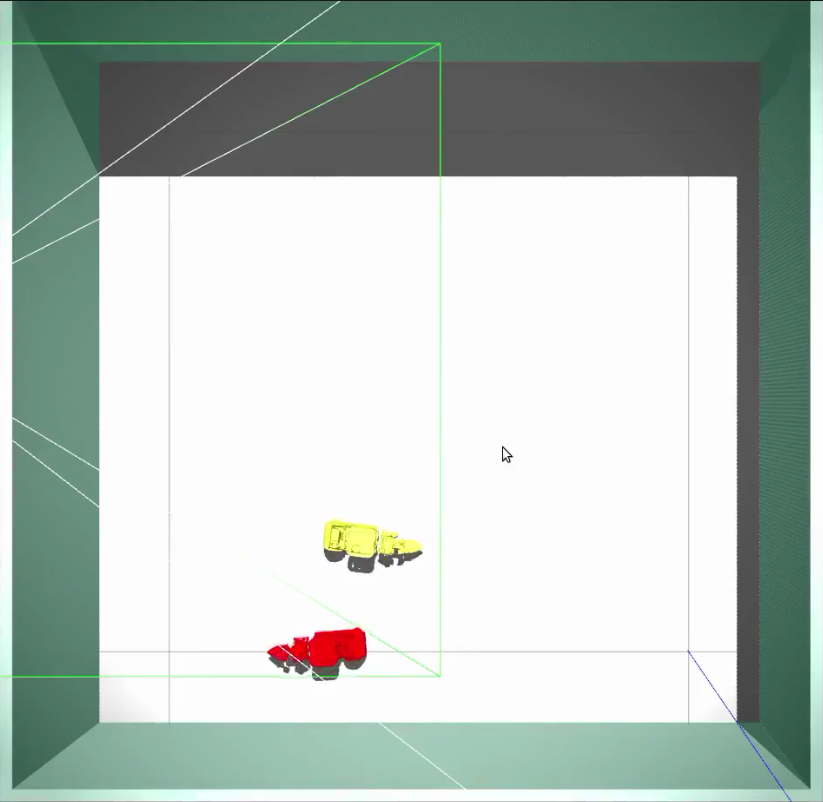
\includegraphics[height=2.5cm]{images/ch05/start/t11.png}
  }
  \subfigure[$t=20~s$]{\label{figure_startdirectionchange20}
  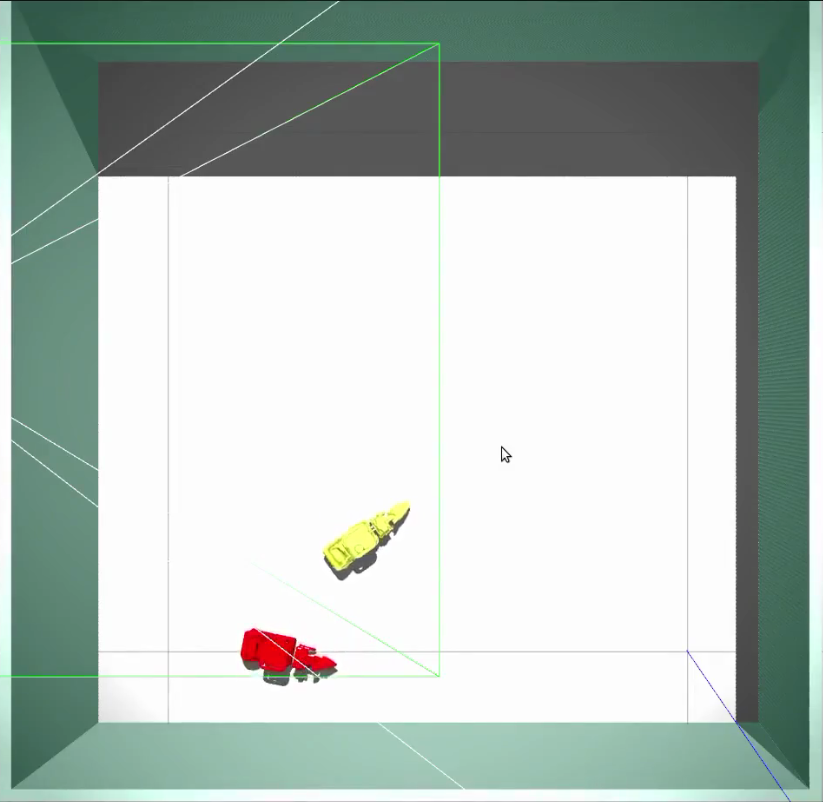
\includegraphics[height=2.5cm]{images/ch05/start/t20.png}
  }
  \subfigure[$t=31~s$]{\label{figure_startdirectionchange31}
  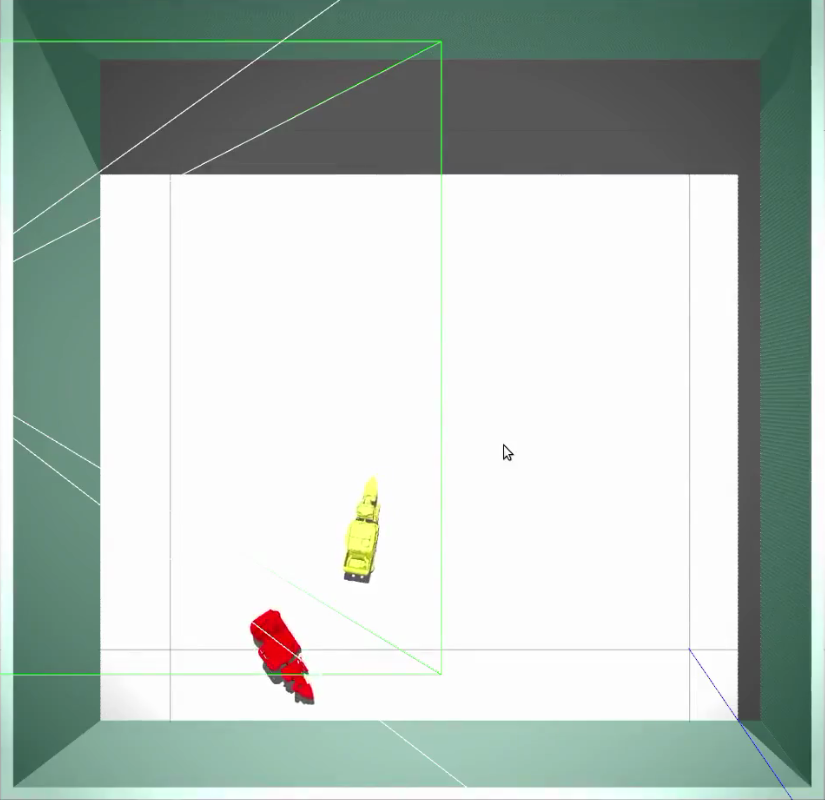
\includegraphics[height=2.5cm]{images/ch05/start/t31.png}
  }\\
  \subfigure[$t=42~s$,被梳理]{\label{figure_actionchange42}
  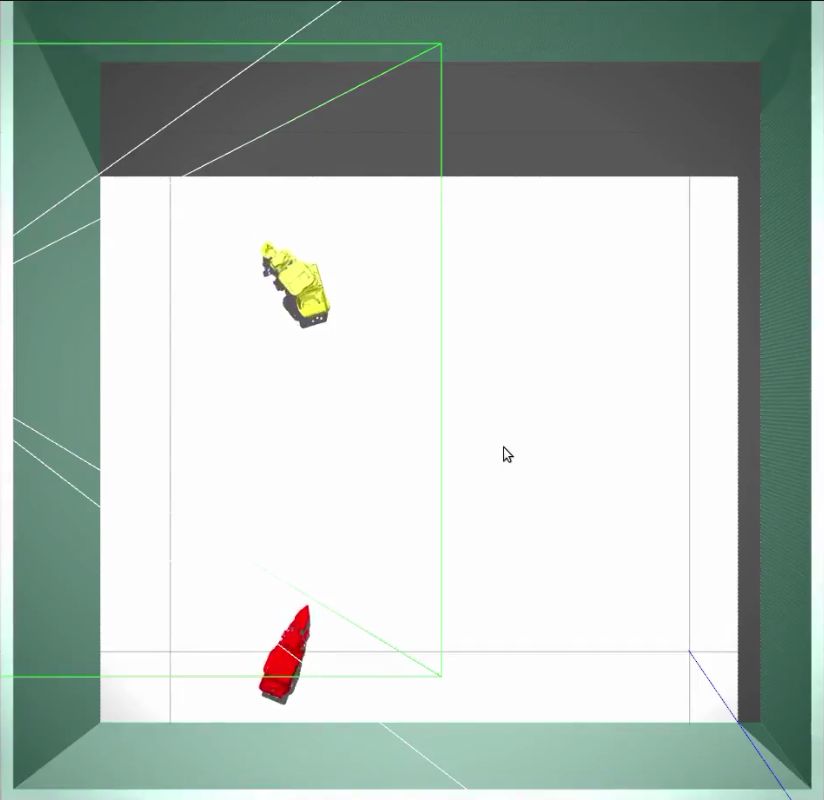
\includegraphics[height=2.5cm]{images/ch05/start/t42.png}
  }
  \subfigure[$t=52~s$,梳理]{\label{figure_actionchange52}
  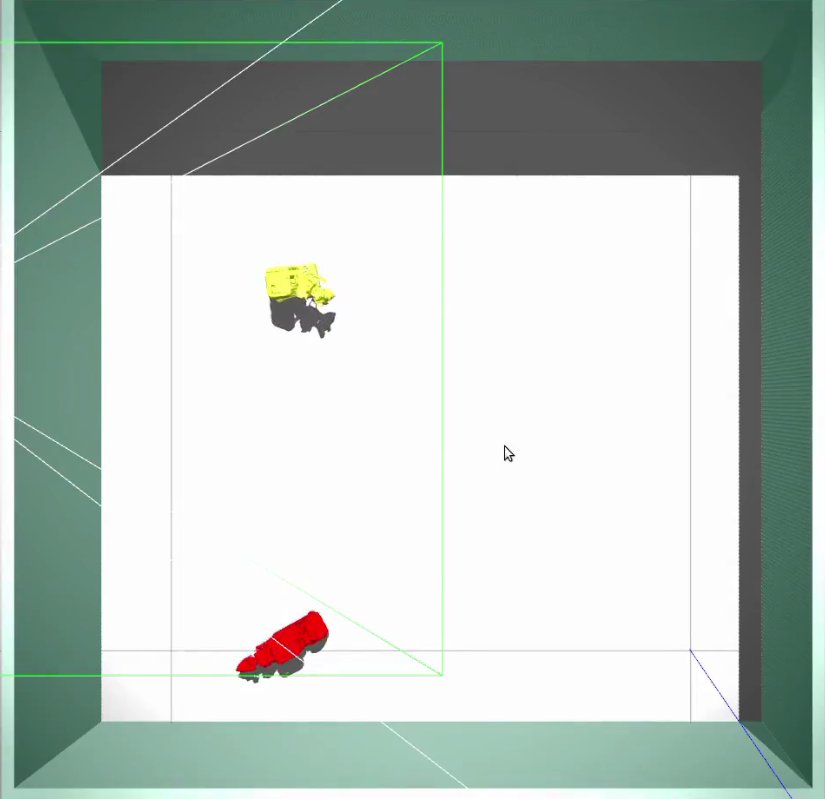
\includegraphics[height=2.5cm]{images/ch05/start/t52.png}
  }
  \subfigure[$t=56~s$,攀爬]{\label{figure_actionchange56}
  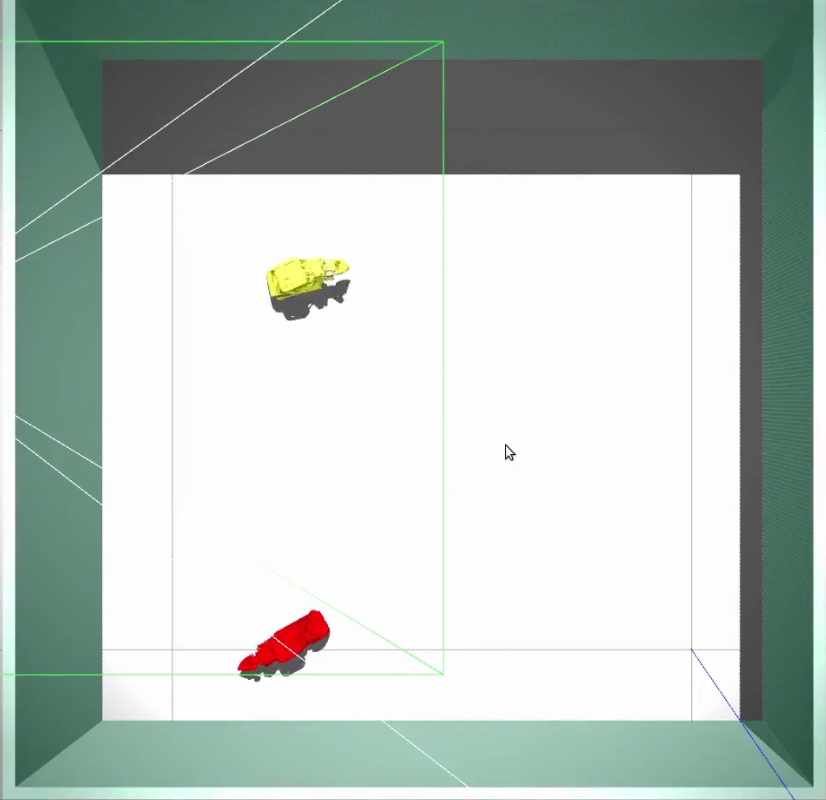
\includegraphics[height=2.5cm]{images/ch05/start/t56.png}
  }
  \caption{训练开始阶段学习鼠的动作尝试}\label{figure_startdirectionchange}
\end{figure}

学习鼠在这一阶段存在两处停留时间较长的地点,这期间进行了一系列动作尝试。在$11\sim32~s$和$40\sim60~s$这两个时间段内,学习鼠在原地进行了多次方向调整,同时产生了包括被梳理、梳理和攀爬等动作(图\ref{figure_startdirectionchange})。但这些尝试并未引起规则鼠的交互反应,未能达到友好交互的状态。

将仿真过程中规则鼠与学习鼠中心的距离$d_{cc}$作为指标,图\ref{figure_roboticdistance}反映了图\ref{figure_roboticheatmap}中的$1~min$内这一指标的变化情况,最短距离为$0.24~m$,出现在$t=11~s$时刻。根据学习鼠的状态划分原则,这一阶段的学习鼠与规则鼠极少进入有效交互距离以内($d_{cc}<0.3~m$)。
\begin{figure}[htbp]
  \vspace{13pt}
  \centering
  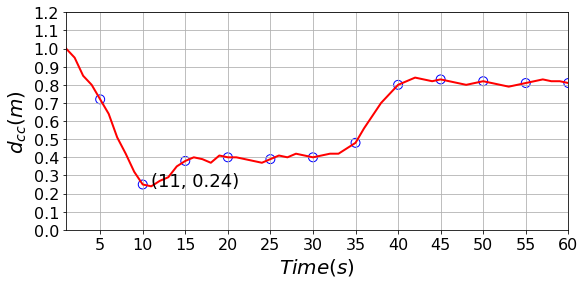
\includegraphics[height=6cm]{images/ch05/start/distance.png}
  \caption{训练开始阶段机器鼠中心距离($1~min$)}\label{figure_roboticdistance}
\end{figure}

即便在$11\sim13~s$内,虽然距离足够进行行为交互,但此时二者并未做出相应的动作(图\ref{figure_start10-13})。
\begin{figure}[htbp]
  \vspace{13pt}
  \centering
  \subfigure[$t=10~s$]{\label{figure_start10}
  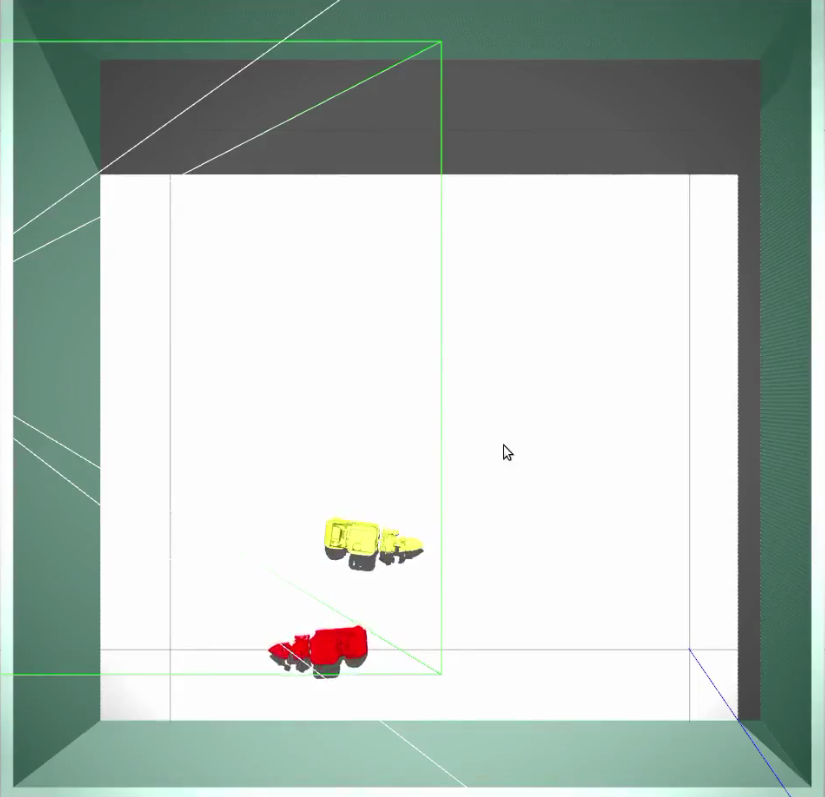
\includegraphics[height=2.5cm]{images/ch05/start/t10.png}
  }
  \subfigure[$t=11~s$]{\label{figure_start11}
  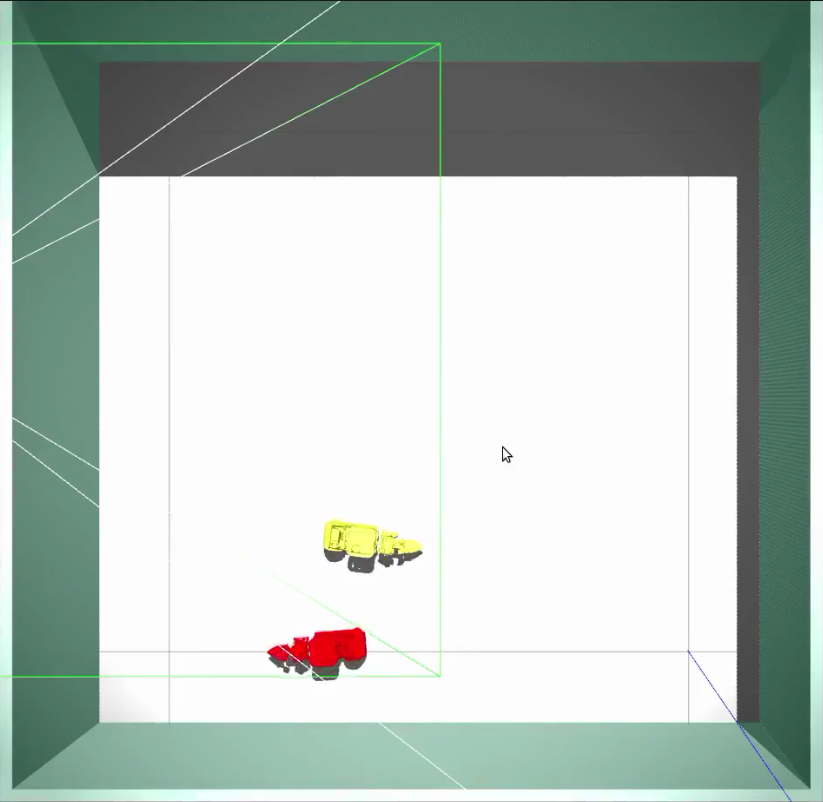
\includegraphics[height=2.5cm]{images/ch05/start/t11.png}
  }
  \subfigure[$t=12~s$]{\label{figure_start12}
  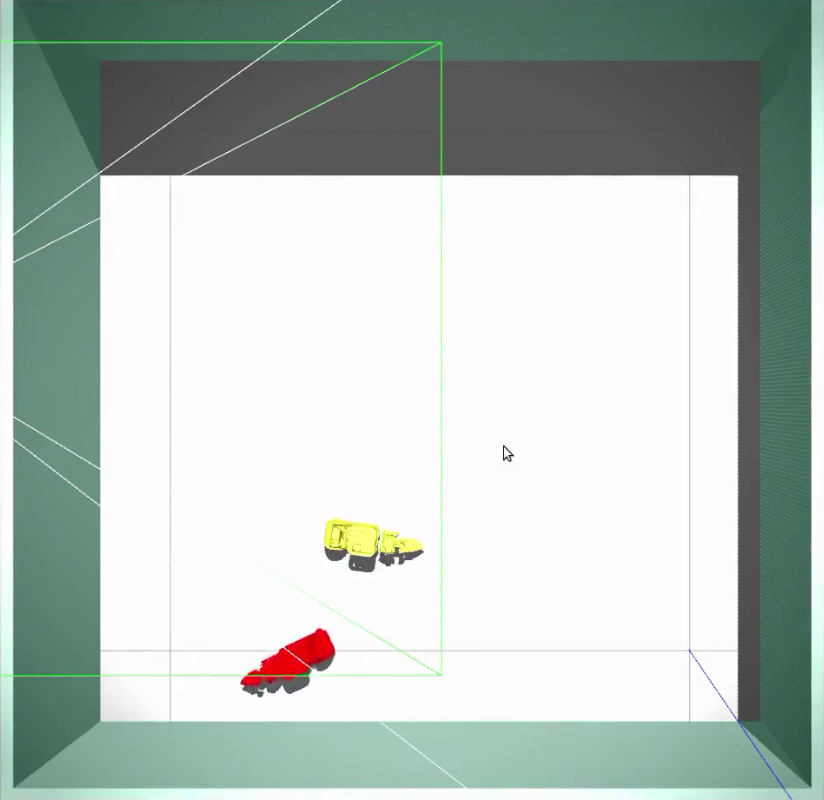
\includegraphics[height=2.5cm]{images/ch05/start/t12.png}
  }
  \subfigure[$t=13~s$]{\label{figure_start13}
  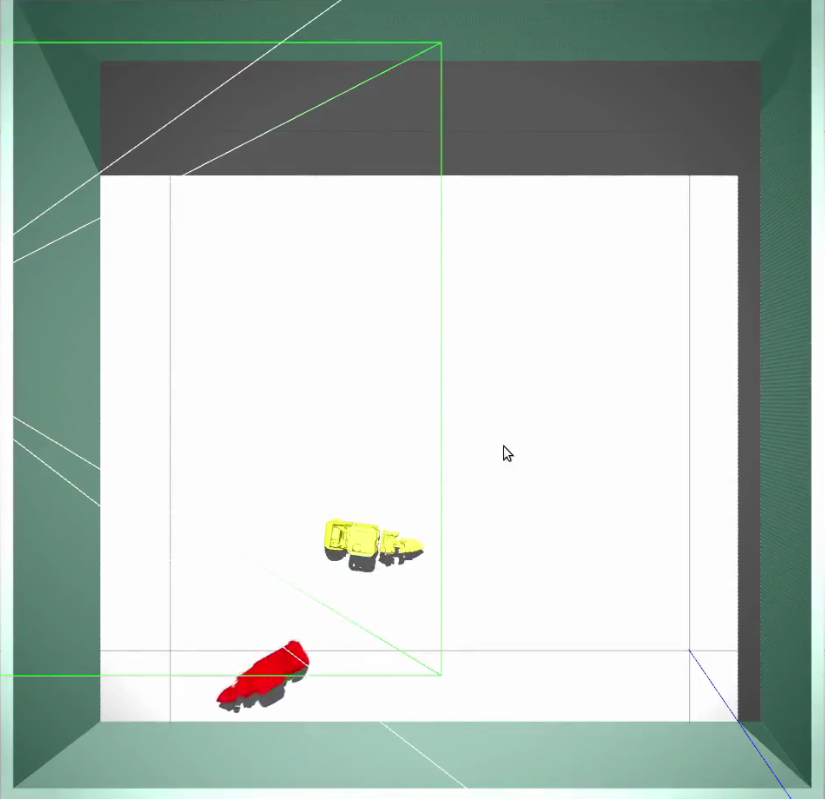
\includegraphics[height=2.5cm]{images/ch05/start/t13.png}
  }
  \caption{$10\sim13~s$内学习鼠与规则鼠动作表现}\label{figure_start10-13}
\end{figure}

%对这一阶段学习鼠各动作的产生频次进行统计
上述分析表明,在学习鼠训练初期,其行为决策主要基于对环境的探索。这一阶段,学习鼠将尽可能尝试所有的状态-动作组以期获得正向即时奖励。而对规则鼠而言,由于缺乏交互对象的积极回应和相应的提高其交互欲望的动作表现,其进行行为交互的尝试也无法成功。
